% figures-es/value-spine.tex
% Standalone TikZ: espina de creación de valor — nueve etapas del libro como cadena de izquierda a derecha (ch.32).
\documentclass[tikz,border=6pt]{standalone}
\usepackage{tikz}
\usetikzlibrary{arrows.meta,positioning,calc}

\definecolor{vcblue}{HTML}{1A5276}
\definecolor{vcteal}{HTML}{0E6655}
\definecolor{vcgrey}{HTML}{5D6D7E}

\begin{document}
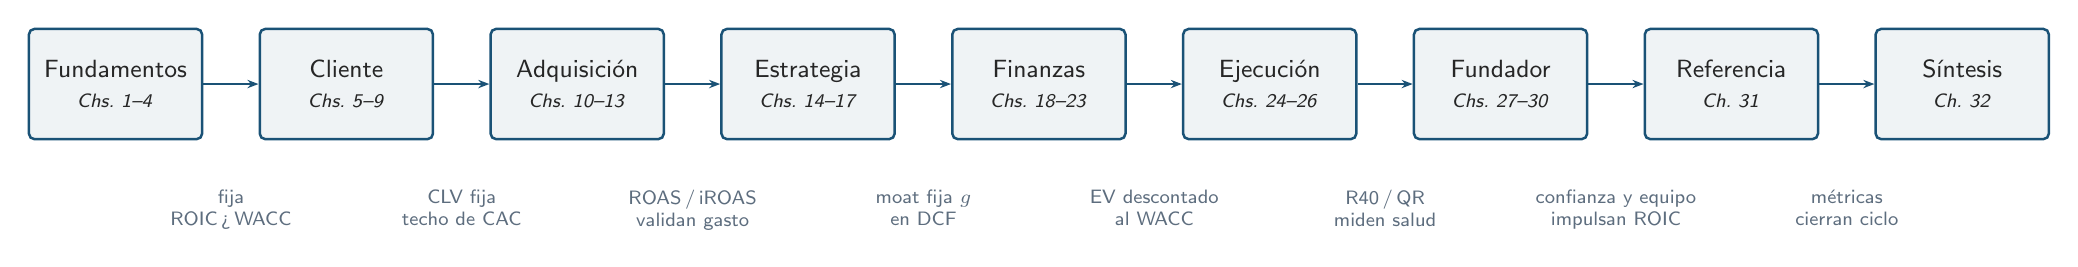
\begin{tikzpicture}[
  node distance=7mm,
  stage/.style={draw=vcblue, line width=0.9pt, rounded corners=2pt, fill=vcblue!7,
                font=\sffamily\small, align=center,
                minimum width=22mm, minimum height=14mm, text=black!85},
  arrow/.style={-{Stealth[length=4pt]}, vcblue, line width=0.9pt},
  ann/.style={font=\sffamily\scriptsize, text=vcgrey, align=center},
]

  %% Nodos de izquierda a derecha
  \node[stage] (found) {Fundamentos\\{\scriptsize\sffamily\textit{Chs.\ 1--4}}};
  \node[stage, right=7mm of found] (cust) {Cliente\\{\scriptsize\sffamily\textit{Chs.\ 5--9}}};
  \node[stage, right=7mm of cust] (acq)  {Adquisición\\{\scriptsize\sffamily\textit{Chs.\ 10--13}}};
  \node[stage, right=7mm of acq]  (strat){Estrategia\\{\scriptsize\sffamily\textit{Chs.\ 14--17}}};
  \node[stage, right=7mm of strat](fin)  {Finanzas\\{\scriptsize\sffamily\textit{Chs.\ 18--23}}};
  \node[stage, right=7mm of fin]  (exec) {Ejecución\\{\scriptsize\sffamily\textit{Chs.\ 24--26}}};
  \node[stage, right=7mm of exec] (fdr)  {Fundador\\{\scriptsize\sffamily\textit{Chs.\ 27--30}}};
  \node[stage, right=7mm of fdr]  (ref)  {Referencia\\{\scriptsize\sffamily\textit{Ch.\ 31}}};
  \node[stage, right=7mm of ref]  (cap)  {Síntesis\\{\scriptsize\sffamily\textit{Ch.\ 32}}};

  %% Flechas de la cadena principal
  \draw[arrow] (found.east) -- (cust.west);
  \draw[arrow] (cust.east)  -- (acq.west);
  \draw[arrow] (acq.east)   -- (strat.west);
  \draw[arrow] (strat.east) -- (fin.west);
  \draw[arrow] (fin.east)   -- (exec.west);
  \draw[arrow] (exec.east)  -- (fdr.west);
  \draw[arrow] (fdr.east)   -- (ref.west);
  \draw[arrow] (ref.east)   -- (cap.west);

  %% Anotaciones debajo de cada flecha (qué alimenta cada etapa)
  \node[ann, below=5mm of $(found.south east)!0.5!(cust.south west)$]
    {fija\\ROIC\,>\,WACC};
  \node[ann, below=5mm of $(cust.south east)!0.5!(acq.south west)$]
    {CLV fija\\techo de CAC};
  \node[ann, below=5mm of $(acq.south east)!0.5!(strat.south west)$]
    {ROAS\,/\,iROAS\\validan gasto};
  \node[ann, below=5mm of $(strat.south east)!0.5!(fin.south west)$]
    {moat fija $g$\\en DCF};
  \node[ann, below=5mm of $(fin.south east)!0.5!(exec.south west)$]
    {EV descontado\\al WACC};
  \node[ann, below=5mm of $(exec.south east)!0.5!(fdr.south west)$]
    {R40\,/\,QR\\miden salud};
  \node[ann, below=5mm of $(fdr.south east)!0.5!(ref.south west)$]
    {confianza y equipo\\impulsan ROIC};
  \node[ann, below=5mm of $(ref.south east)!0.5!(cap.south west)$]
    {métricas\\cierran ciclo};

\end{tikzpicture}
\end{document}
